\section{A New Classification} \label{sec:Serotype_Classification}

\begin{figure}[!hbt]
    \centering
    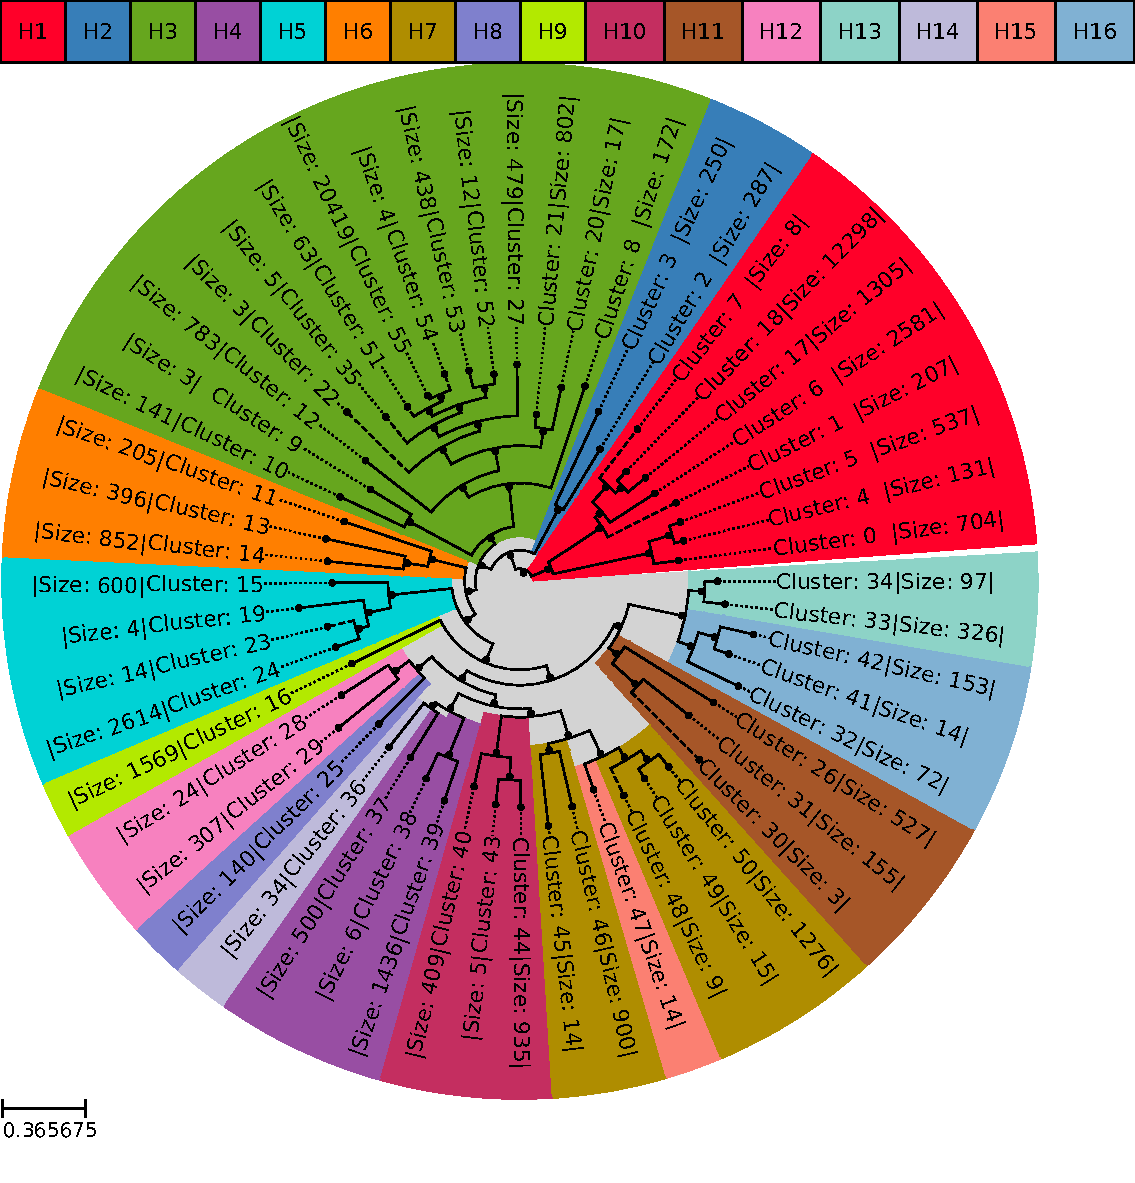
\includegraphics[width=\textwidth]{Results/Clustertree_Segment_4.pdf}
    \caption[Segment 4 cluster tree of k-mer frequency vectors reduced by enhanced \texttt{PCA}]{\textbf{Segment 4 cluster tree of k-mer frequency vectors reduced by enhanced \texttt{PCA}.} The cluster tree of segment 4 clustering, using the combination of \texttt{PCA} and the Kneedle Algorithm (PK) with a reduction to 50 instead of 30 dimensions (\autoref{fig:PCA_Cluster_Knee_4}). The coloring of the clusters in the tree is based on the subtype of the contained sequences. Unclassified sequences of a cluster are reclassified as a given subtype if sequences of only this subtype are present in the cluster in addition to the unclassified ones. Uncolored clusters contain sequences from at least two subtypes and zero or more unclassified sequences. Dotted lines in the tree indicate the same host.}
    \label{fig:Result_Clustertree_Segment_4}
\end{figure}

Reannotation of the most likely false annotated sequences in \autoref{fig:PCA_Clusteree_Knee_4} \textbf{\textsf{C}} as well as increasing of the components in \texttt{PCA} successfully raised the accuracy of the pipeline. Clustering errors found in the previous section were resolved successfully as H13 and H16 are now completely divided, with the mentioned small but still present difference between these subtypes. Also, all clusters of H3 are now present in direct connection to each other and no cluster not homogeneous for one subtype exist anymore. 

Resulting from this improved clustering of segment 4 a new classification involving 56 groups instead of 18 subtypes is proposed (\autoref{fig:Result_Clustertree_Segment_4}).
%neue classification vorschlagen blablabla
% vielleicht bisschen evolution black sea gull etc

By pairwise comparison of random 10 sequence samples of these groups the similarity inside these groups is described in \autoref{fig:Proof_Clustertree_Segment_4}. To avoid creating a bias, the result for accidental comparisons of sequences with the same accession are ignored and not considered in calculations of respective mean values.

\begin{figure}[!hbt]
    \centering
    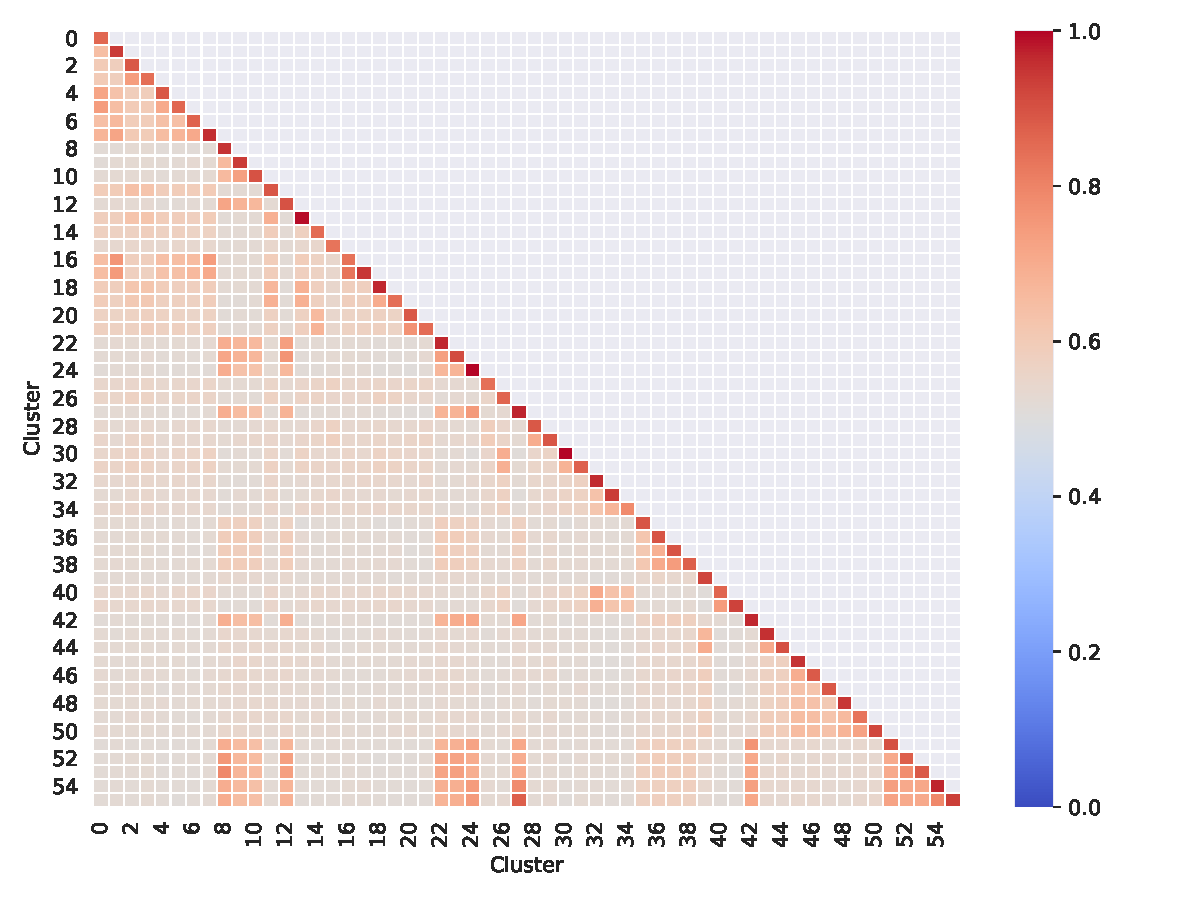
\includegraphics[width=\textwidth]{Results/Cluster_Difference_Segment_4.pdf}
    \caption[Sample sequence similarity matrix of segment 4 clusters]{\textbf{Sample sequence similarity matrix of segment 4 clusters.}. Random samples of up to 10 sequences of every cluster in \autoref{fig:Result_Clustertree_Segment_4} were compared by pairwise alignments with the samples of all other clusters. Less than 10 sequences were only used in clusters containing less than 10 sequences. The percentage of similarity was calculated for very alignment making a matrix of up to $10\times10$ holding the similarity values of the samples comparisons. The mean of the matrix was then calculated and written as the given cluster interactions mean similarity. This was repeated for every possible cluster interaction resulting in the presented figure. Interactions of the same clusters were reduced to only different sequences, results of alignments with sequences having the same accession were removed, thereby, preventing bias creation. The mean of these up to 100 comparisons for every cluster interaction are colored according to their similarity from 1.0 or 100\% similarity in red to 0.0 or 0\% similarity in blue.}
    \label{fig:Proof_Clustertree_Segment_4}
\end{figure}

All clusters in \autoref{fig:Proof_Clustertree_Segment_4} have the highest similarities with themselves and mostly high similarities with clusters of the same subtype. For instance cluster 0, share some degree of sequence identity with other clusters stemming from the same subtype H1, as shown in \autoref{fig:Proof_Clustertree_Segment_4}. However, the highest similarity of around 90\% is only shared with other sequences of the cluster itself, which makes this cluster very self contained. 

Exceptions for the relative high similarity to other clusters of the same subtypes are the subtypes H7 and H15 with the clusters 45 to 50, as well as H4 and H14 with clusters 35 to 38. There was no clear separation performed as the clusters merge with other subtypes in higher tree nodes, although other clusters of the same subtype are still available (\autoref{fig:Result_Clustertree_Segment_4}). The similarities of these cluster, are also high compared to the other subtype and indicate a relation neglected by the subtype classification. The almost uniform H7 subtree of clusters 45, 46, 48, 49, and 50 is divided by the one and only cluster of subtype H15 cluster 47. When comparing the sequence similarities in \autoref{fig:Proof_Clustertree_Segment_4}, the highest similarity persist inside the clusters themselves, but the cross similarities of cluster 45 and 46 to 47, 48, 49, and 50 are around 65\% without big difference between subtype H7 and H15.  

With this pipeline blueprint created by adjusting the clustering for segment 4, all \gls{IAV} segments could be clustered the same way, since no subtype information is necessary for the clustering. Coloring of the tree was performed as guideline and was the only part involving actual sequence subtype evaluation. Thereby, the cluster trees for most other segments are uncolored. All other cluster trees and similarity matrix graphics, as well as tables containing sequence cluster assignment and the tables containing the values used to create the graphics are presented in the \autoref{chap:Appendix}. Hereby new classifications for all segments based on k-mer frequency are proposed, containing 28 groups for segment one, 28 for two, 29 for three, the shown 57 for segment 4, 26 for five, 40 for six, 30 for seven and 24 groups for segment eight. 

The groups of the segments one to three, five, seven, and eight share by far more overall similarity, therefore, less clusters were created. Still, the similarity inside the clusters themselves is higher than the cross similarity and, thereby, solid clustering by the proposed clustering method was possible despite the overall higher similarity (\autoref{chap:Appendix}). 

Present day research propose a phylogenetic tree of \gls{IAV} that is split in four subtrees \autocite{wei_next-generation_2020}. 

Alignment evoltion not used in kmer maybe acknowledge evol dist in kmer 